

\chapter{Background} \label{section:background}
This chapter provides an overview of the background knowledge relevant for the thesis. First, a general overview of Moving Target Defence (\acrshort{mtd}) is introduced. Second, some background information on IoT security is presented. This includes some architectural information as well as common IoT malware and how they work. A subsection on cooperative defence concludes the chapter.

\section{General Overview of Moving Target Defense} \label{section:MTD}
Although the idea of modifying system components to prevent others from disrupting the systems has been around for some time, the first use of the term "MTD" was proposed in 2009 by Networking and Information Technology Research and Development (NITRD)~\cite{navas:2021MTDWhere}. The following paragraph is based on this very NITRD source~\cite{report:GhoshMovingTargetDefense}, which despite its age serves as a good overview of MTD.  

One of the main problems of systems is their relatively static configuration. This static design stems from the fact that, in the past, system requirements focused on simplicity and elegance rather than security, as exploitation of vulnerabilities was not a concern. An example are IP addresses and other configuration parameters that remain static over a relatively long period of time. An adversary needs to know the vulnerabilities of a system in order to attack it effectively. The longer the vulnerabilities exist, the more likely they are to be exploited. Therefore, a static system is a significant advantage for an adversary because it gives them enough time to prepare and plan their attack. This is the motivation behind MTD, which involves building systems that change rapidly to minimise the likelihood of a successful attack. 
%A key challenge for MTD is to ensure that the system remains maintainable and reliable for its users. There is no point in having a secure system if it is not usable and reliable. 

Another great and more recent summary was given by~\cite{navas:2021MTDWhere}. Since system information does not expire, an attacker with enough resources (e.g. time) will ultimately find a vulnerability and succeed in his attack. MTD tries to increase the resources needed for an attacker to succeed by continuously altering the attack surface of the system. The sum of a system's vulnerabilities can be defined as its attack surface~\cite{website:IBMAttack}. 



\cite{article:Cai} concluded from the existing literature that three elements must be defined for an MTD technique to achieve the defence objective. 
\begin{enumerate}
    \item \textbf{What to move}: This defines the moving parameter (MP), which is an essential attribute (e.g. IP address or service port) of an attack target. Each MP has a domain from which its values can be selected. 
    \item \textbf{How to move}: This describes how the MP should be moved. This involves selecting a new MP value from its range and replacing the old MP value. There are several ways to choose the new value, such as randomly, game theoretically or situationally.   
    \item \textbf{When to move}: This describes the frequency with which the current value of the MP should be replaced by the new one. This is a critical element because if the MP changes too often, it could lead to poor system performance; if it changes too little, an attacker could be successful.~\cite{navas:2021MTDWhere} identified three different decision processes in the literature: time-based, event-based and hybrid.
\end{enumerate}


\cite{article:okhraviFindingFocus} reviewed five dominant domains of MTD techniques, including the advantages and disadvantages of each. Below is a presentation of these 5 domains. For each domain,~\cite{article:okhraviFindingFocus} also indicated the phase of the attack that the domain seeks to disrupt. For this, the authors chose a five-phase attack consisting of the following phases: 
\begin{itemize}
    \item Reconnaissance: This phase is mainly limited to observation, where the attacker tries to find a target and collect basic information about it. An example of this is finding the IP address of a host through IP scanning.
    \item Access: In this phase, the adversaries collect detailed information about their target. In the case of e.g. a web server, this could include its operating system or configuration. 
    \item Development: In this phase, the adversaries develop an attack that targets a previously found vulnerability. This can be achieved offline without any connection to the target. 
    \item Launch: In this phase, the adversaries compromise the target by delivering the attack payload. This can be done in a variety of ways, including infected media or over the network.
    \item Persistence: If the adversaries wish to remain in the compromised system, they can install additional entry points into the system, such as backdoors. 
\end{itemize}

Each of the MTD domains described below attempts to disrupt one or more of these phases. This is only an overview of the domains and does not cover specific techniques~\cite{article:okhraviFindingFocus}.     

\subsection{Dynamic Networks}
MTD techniques in this domain modify network properties to increase the required workload for an attacker and thus reduce the probability of a successful attack. These techniques are primarily used to prevent the success of the reconnaissance phase, but can also be used to prevent a successful launch phase. Possible means to achieve these network modifications include frequent address and port changes, or changing the logical network topology. The logical network topology is how devices are arranged in a computer network and how they communicate with each other~\cite{article:Santra2013}. 

One problem with such techniques is that they may hinder convenient use of the system when applied to a service of a system that needs to remain in a known network location. An example are public servers, where such a technique would defeat its purpose as the server would be hidden even for legitimate users. Another challenge is that the degree of uncertainty created for attackers is critical to the effectiveness of randomization. Entropy, a value that depends on the number of possible values and their corresponding probabilities, can measure the uncertainty in a random value, but this entropy is limited in many dynamic network techniques. One reason for this is that IP addresses and port numbers can be limited by the network infrastructure.  


\subsection{Dynamic Platforms}
MTD techniques in this domain focus on modifying the computing platform characteristics. The goal is the disruption of attacks that depend on specific platform properties. There are several properties that can be changed, such as the operating system, storage systems, virtual machine instances, or communication channels. It is possible for the same application to run in parallel in different architectural contexts, or for applications to migrate from machine to machine. In terms of attack phases, these techniques provide protection in all five phases, but are most beneficial in the access, development and persistence phases. This is because an attack is much more difficult if it requires exploits for multiple platforms to succeed. This is especially true if the program is executed in parallel on several instances. 

A problem with dynamic platforms is that these techniques also increase the attack surface because additional code is used to control and manage migrations. Additionally, an attacker may gain an advantage due to a specific vulnerability in the platform on which the application is currently running.   
Another problem with dynamic platforms is that it can be difficult to maintain or synchronise state across platforms in a platform-independent format if required by the application. Even if the state transfer can be performed, care must be taken to ensure that the attacker does not remain in the state, resulting in persistence of the attacker in the system.  


\subsection{Dynamic Runtime Environment}
The goal of dynamic runtime environment techniques is to prevent the exploitation of software vulnerabilities by randomizing the environment in which the application runs. These techniques assume that the attacker already has an exploitable vector, and the techniques are designed to prevent the attack from being executed. One problem that these techniques can prevent is buffer overflow exploits, which can lead to code injection. 
These techniques can be further divided into two sub-domains: Instruction Set Randomization (ISR) and Address Space Randomization (ASR). ISR can take place in the application, the operating system, or the hardware, and its goal is to prevent attackers from predicting how the program will execute. This is done by randomizing the instructions in an application. A specific example of ISR is encrypting instructions at load time and decrypting them just before execution. ASR techniques aim to create a randomized memory layout from a deterministic one. This prevents the possibility of using a known memory address for things like control flow redirection. One of the best known and most widely used runtime techniques is address space layout randomisation (ASLR), which falls into the ASR subdomain. 

Both subdomains have weaknesses, in the case of the ASR subdomain, or more specifically ASLR techniques, it is the fact that typically only a part of the memory of the application is randomized, while the other part remains static. This static part may be sufficient for an attacker to develop a meaningful payload. Another related problem is that only the base address of the memory segment is randomized, but the relative addresses remain unchanged. This means that the attacker can bypass ASLR by using relative addresses. In addition, due to the architectural limitations of the defended system, the randomized memory spaces are often too small, making them vulnerable to brute-force attacks. Regarding ISR, the main weakness is the performance overhead caused by the fact that ISR techniques often rely on software emulations, as there is often no hardware support. There are ISR techniques that depend on low overhead methods as e.g. XOR encryption, but these techniques are weak encryption methods and there is a possibility that the attacker can recover the key to inject correctly encrypted instructions. 


\subsection{Dynamic Software}
The goal of MTD techniques in this domain is to diversify the application without changing its functionality. Equivalent program instructions substitute each other, changing various properties such as the internal data structure layout or the sequence of instructions. This reduces the likelihood of a successful attack, as the attacker must correctly guess the software variant being used. These techniques aim to disrupt the attacks' development and launch phase by creating uncertainty and making code injection and code reuse more difficult. There are several ways to apply these techniques, either by using an application that has its own internal randomization capability, or by creating multiple semantically equivalent binaries.

In practice, there was no widespread use of dynamic software techniques in 2014. The examples that did exist were mostly limited to academic and research environments. Unfortunately, no more recent source on the current situation of dynamic software techniques could be found. There are also several weaknesses of these techniques, one of which is that it is complex to ensure that the diversified application provides the same functionality as the original. There is also a lack of scalability, the possibility of unexpected side effects, and the significant performance overhead associated with heavy binary translation and emulation. Finally, many applications are designed for maximum performance, and semantically equivalent applications could reduce this performance.  


\subsection{Dynamic Data}
The goal of the dynamic data domain is to change the internal or external data representation by changing the properties of the data representation, such as syntax or format. Similar to the dynamic software domain, the semantic context should remain unchanged, but the change in data representation should prevent unauthorized use or access to the content. These techniques should also complicate the development and deployment phases of the attack, as attack development is hampered by the need to find an adequate payload for the various data representations. Some of these techniques have their origins in techniques developed against data corruption. One example is a technique where computations are performed on multiple data representations, providing the ability to detect corrupted or malicious input. Figure \ref{fig:differentDataFormats} shows two different data representations with the same semantics. 

These techniques also have weaknesses. One is that most standard binary formats support only one canonical representation, resulting in a lack of diversity in possible data encodings. Another drawback from a practical point of view is that dynamic data techniques increase the effort required for application development as well as runtime performance, since multiple data representations may have to be processed and monitored.




\begin{figure}[tph]
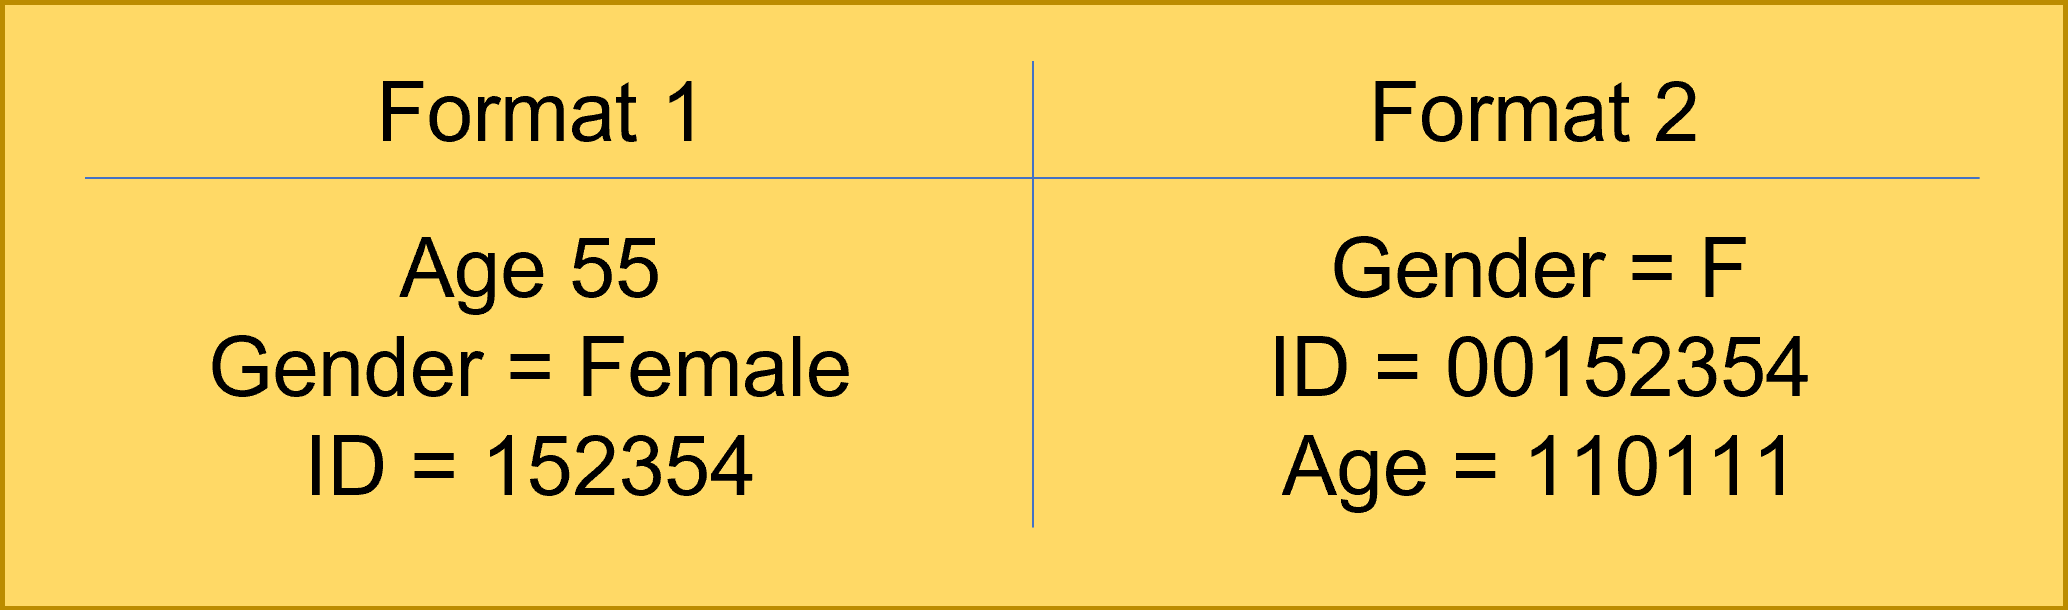
\includegraphics[scale=0.2]{assets/dynamicData.png}
\centering
\caption{Two Different Data Representations With the Same Semantics.}\label{fig:differentDataFormats}
\end{figure}


\subsection{Summary}
Table \ref{table:movingTargetDefense} shows the different moving target defence domains and the corresponding attack phase they seek to disrupt. In their discussion,~\cite{article:okhraviFindingFocus} identified three critical properties for effective MTD, namely unpredictability, comprehensiveness and timeliness. The first property is crucial because if the attacker can predict the next movement of a defence mechanism, the defence becomes obsolete. Comprehensiveness means the inclusion of all elements that could work against an attack, as one element alone may not be very useful. An example is the case where the location of an application's library is randomized, but the application remains in a fixed location. This means that attackers can simply ignore the randomization and attack the fixed code. Timeliness is also important. For example, if attackers can observe the outcome of a moving target defence technique, this knowledge could give them an opportunity to attack. It is also crucial that the attacker is exposed to the diversity of the environment within the attack time. The authors gave an example where an application is migrated among three platforms, so that the attackers would need another vulnerability to continue the attack after the migration to the new platform. However, if the attack time is smaller than the migration time, the security is reduced because the attackers have three different platforms from which to choose vulnerabilities. The authors conclude that some techniques work better for general-purpose environments and some better for specific purposes, as each technique has different strengths and weaknesses.    



\begin{table}[tph]
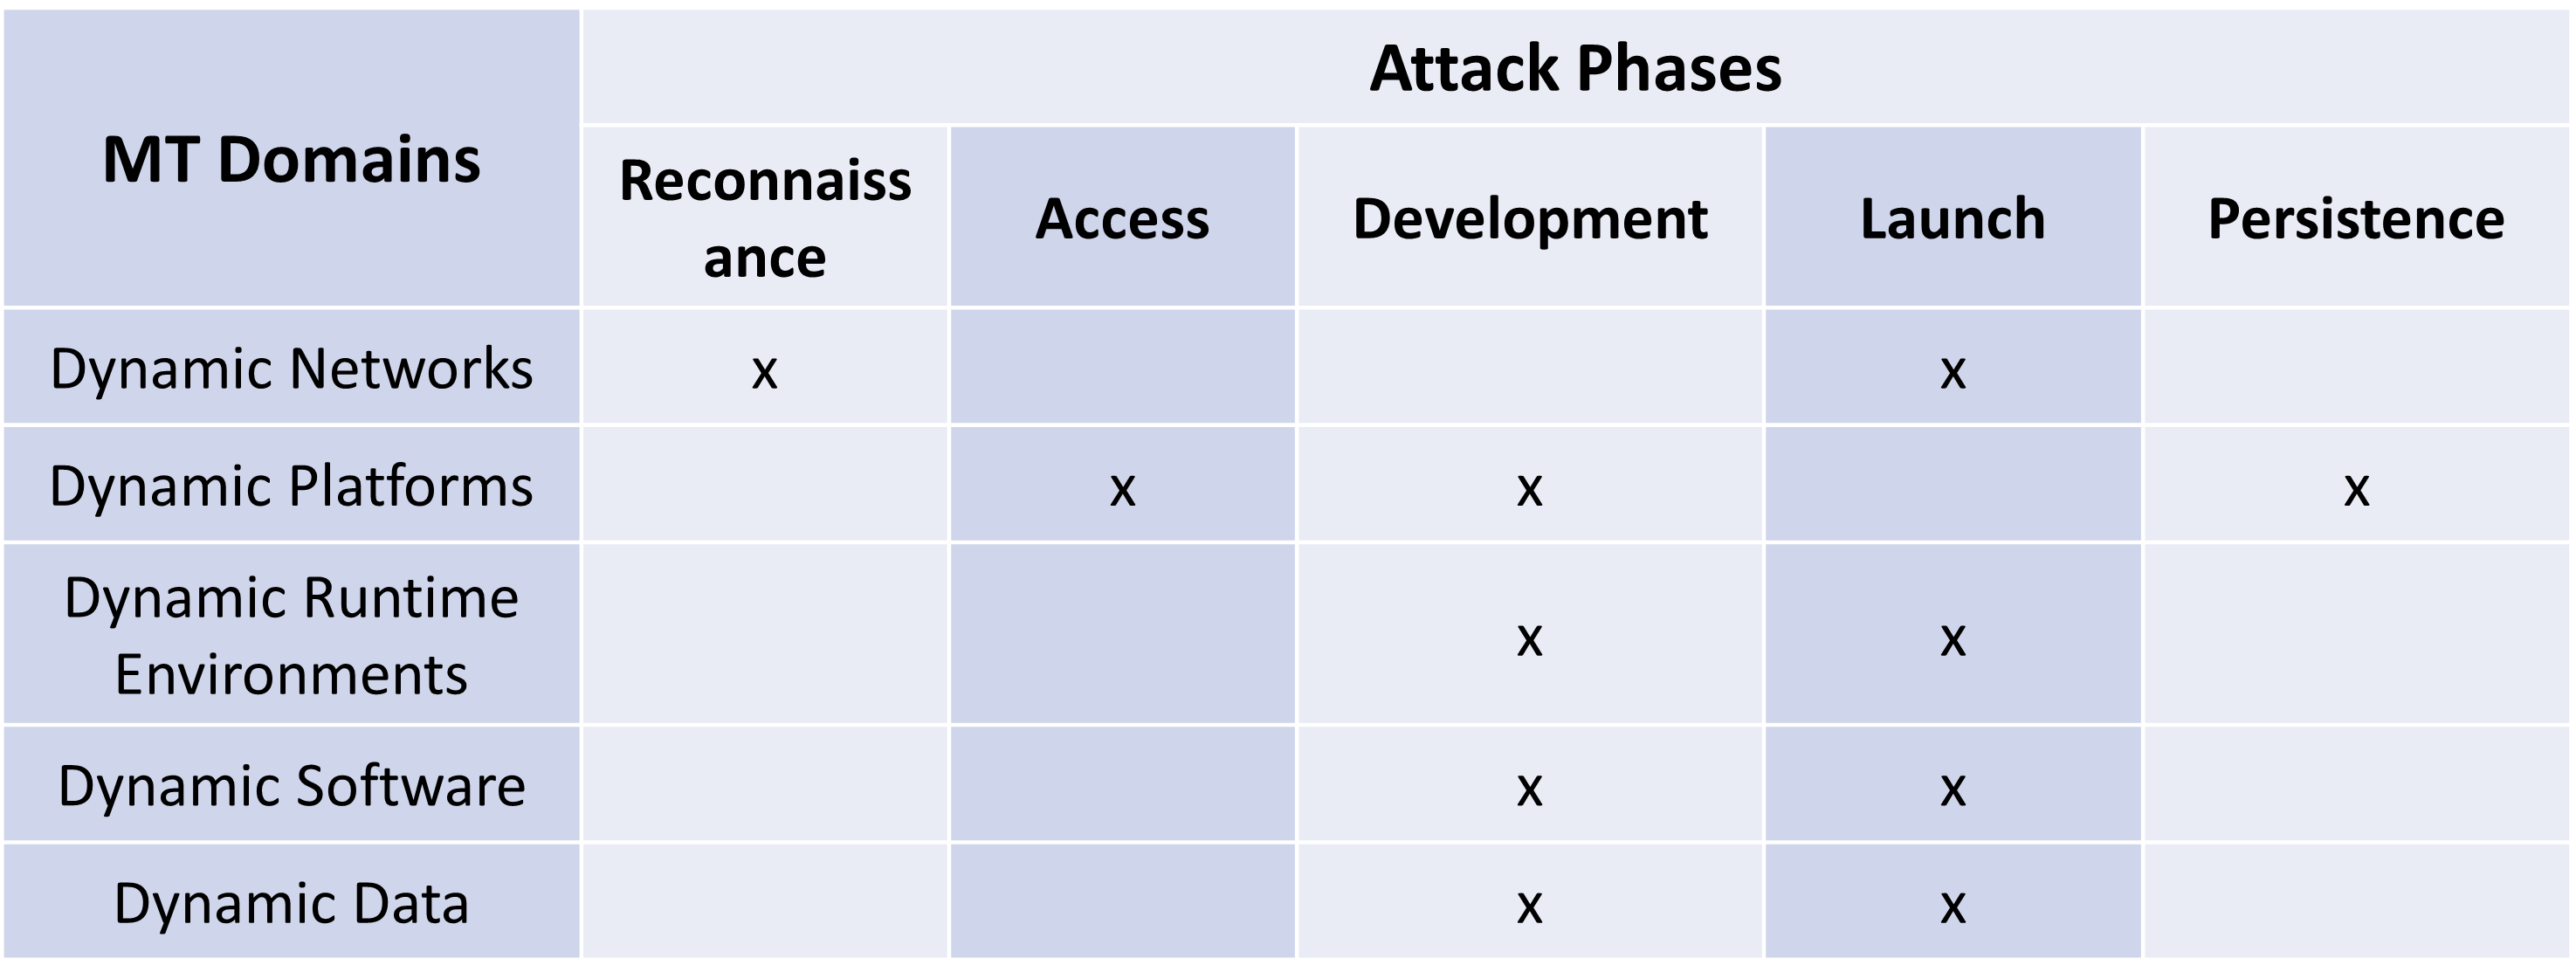
\includegraphics[scale=0.7]{assets/movingTargetDefenseAttack.png}
\centering
\caption{A Summary of the Moving Target Defense Domains and the Corresponding Attack Phase They try to Hinder~\cite{article:okhraviFindingFocus}.}
\label{table:movingTargetDefense}
\end{table}




\section{Internet of Things}
\cite{report:cern} gave a brief introduction about what the Internet of Things (IoT) is. It is about the collection and exchange of data through networked items embedded with electronics, sensors, software, actuators and a network connection. Examples of these items are physical devices, vehicles or buildings. These items can be controlled or sensed across an existing network infrastructure. This enables better integration of the physical world into computer-based systems, which has several benefits, such as reduced need for human intervention and economic benefits. But there are also major challenges for IoT, two of which are security and privacy. For example, a smart meter in a house knows when someone is at home, and this data is also shared with other devices and databases by companies that therefore also have this information.


\subsection{Current and Future Distribution of IoT Devices}
According to~\cite{website:statistaIoT}, there existed 11.3 billion IoT devices worldwide in 2021. By 2030, this number is expected to nearly triple to an estimated 29.3 billion devices.~\cite{website:fortuneIoT} estimated the global market size for IoT from 2022 to 2029. They estimated the market size to be 2,465.26 billion in 2029, which is significantly higher than the current 478.36 billion. Also interesting is the analysis of the current market share by end-use industry. At 21.5\%, the largest share of the end-use industry is accounted for by the healthcare market, followed by the manufacturing market and the IT \& telecom market. These three account for around 50\% of the total market share. Other examples include retail, transportation and banking, financial services and insurance.


\cite{website:gfuSurvery} has published a survey conducted in July 2021 on Smart Home solutions (consisting of IoT devices) and how many users are currently using them and how many users intend to use them in the future. 5 different groups were formed, which are shown in Table \ref{table:IoT}. It can be seen that some groups currently have a higher share and others a lower share, but the intended future use is significantly higher for each group. Another interesting insight is the breadth of the groups, ranging from lamps to security to garden and balcony. Thus, IoT devices can already be found in various places, and they will become even more important than they are today.  

\begin{table}[tph]
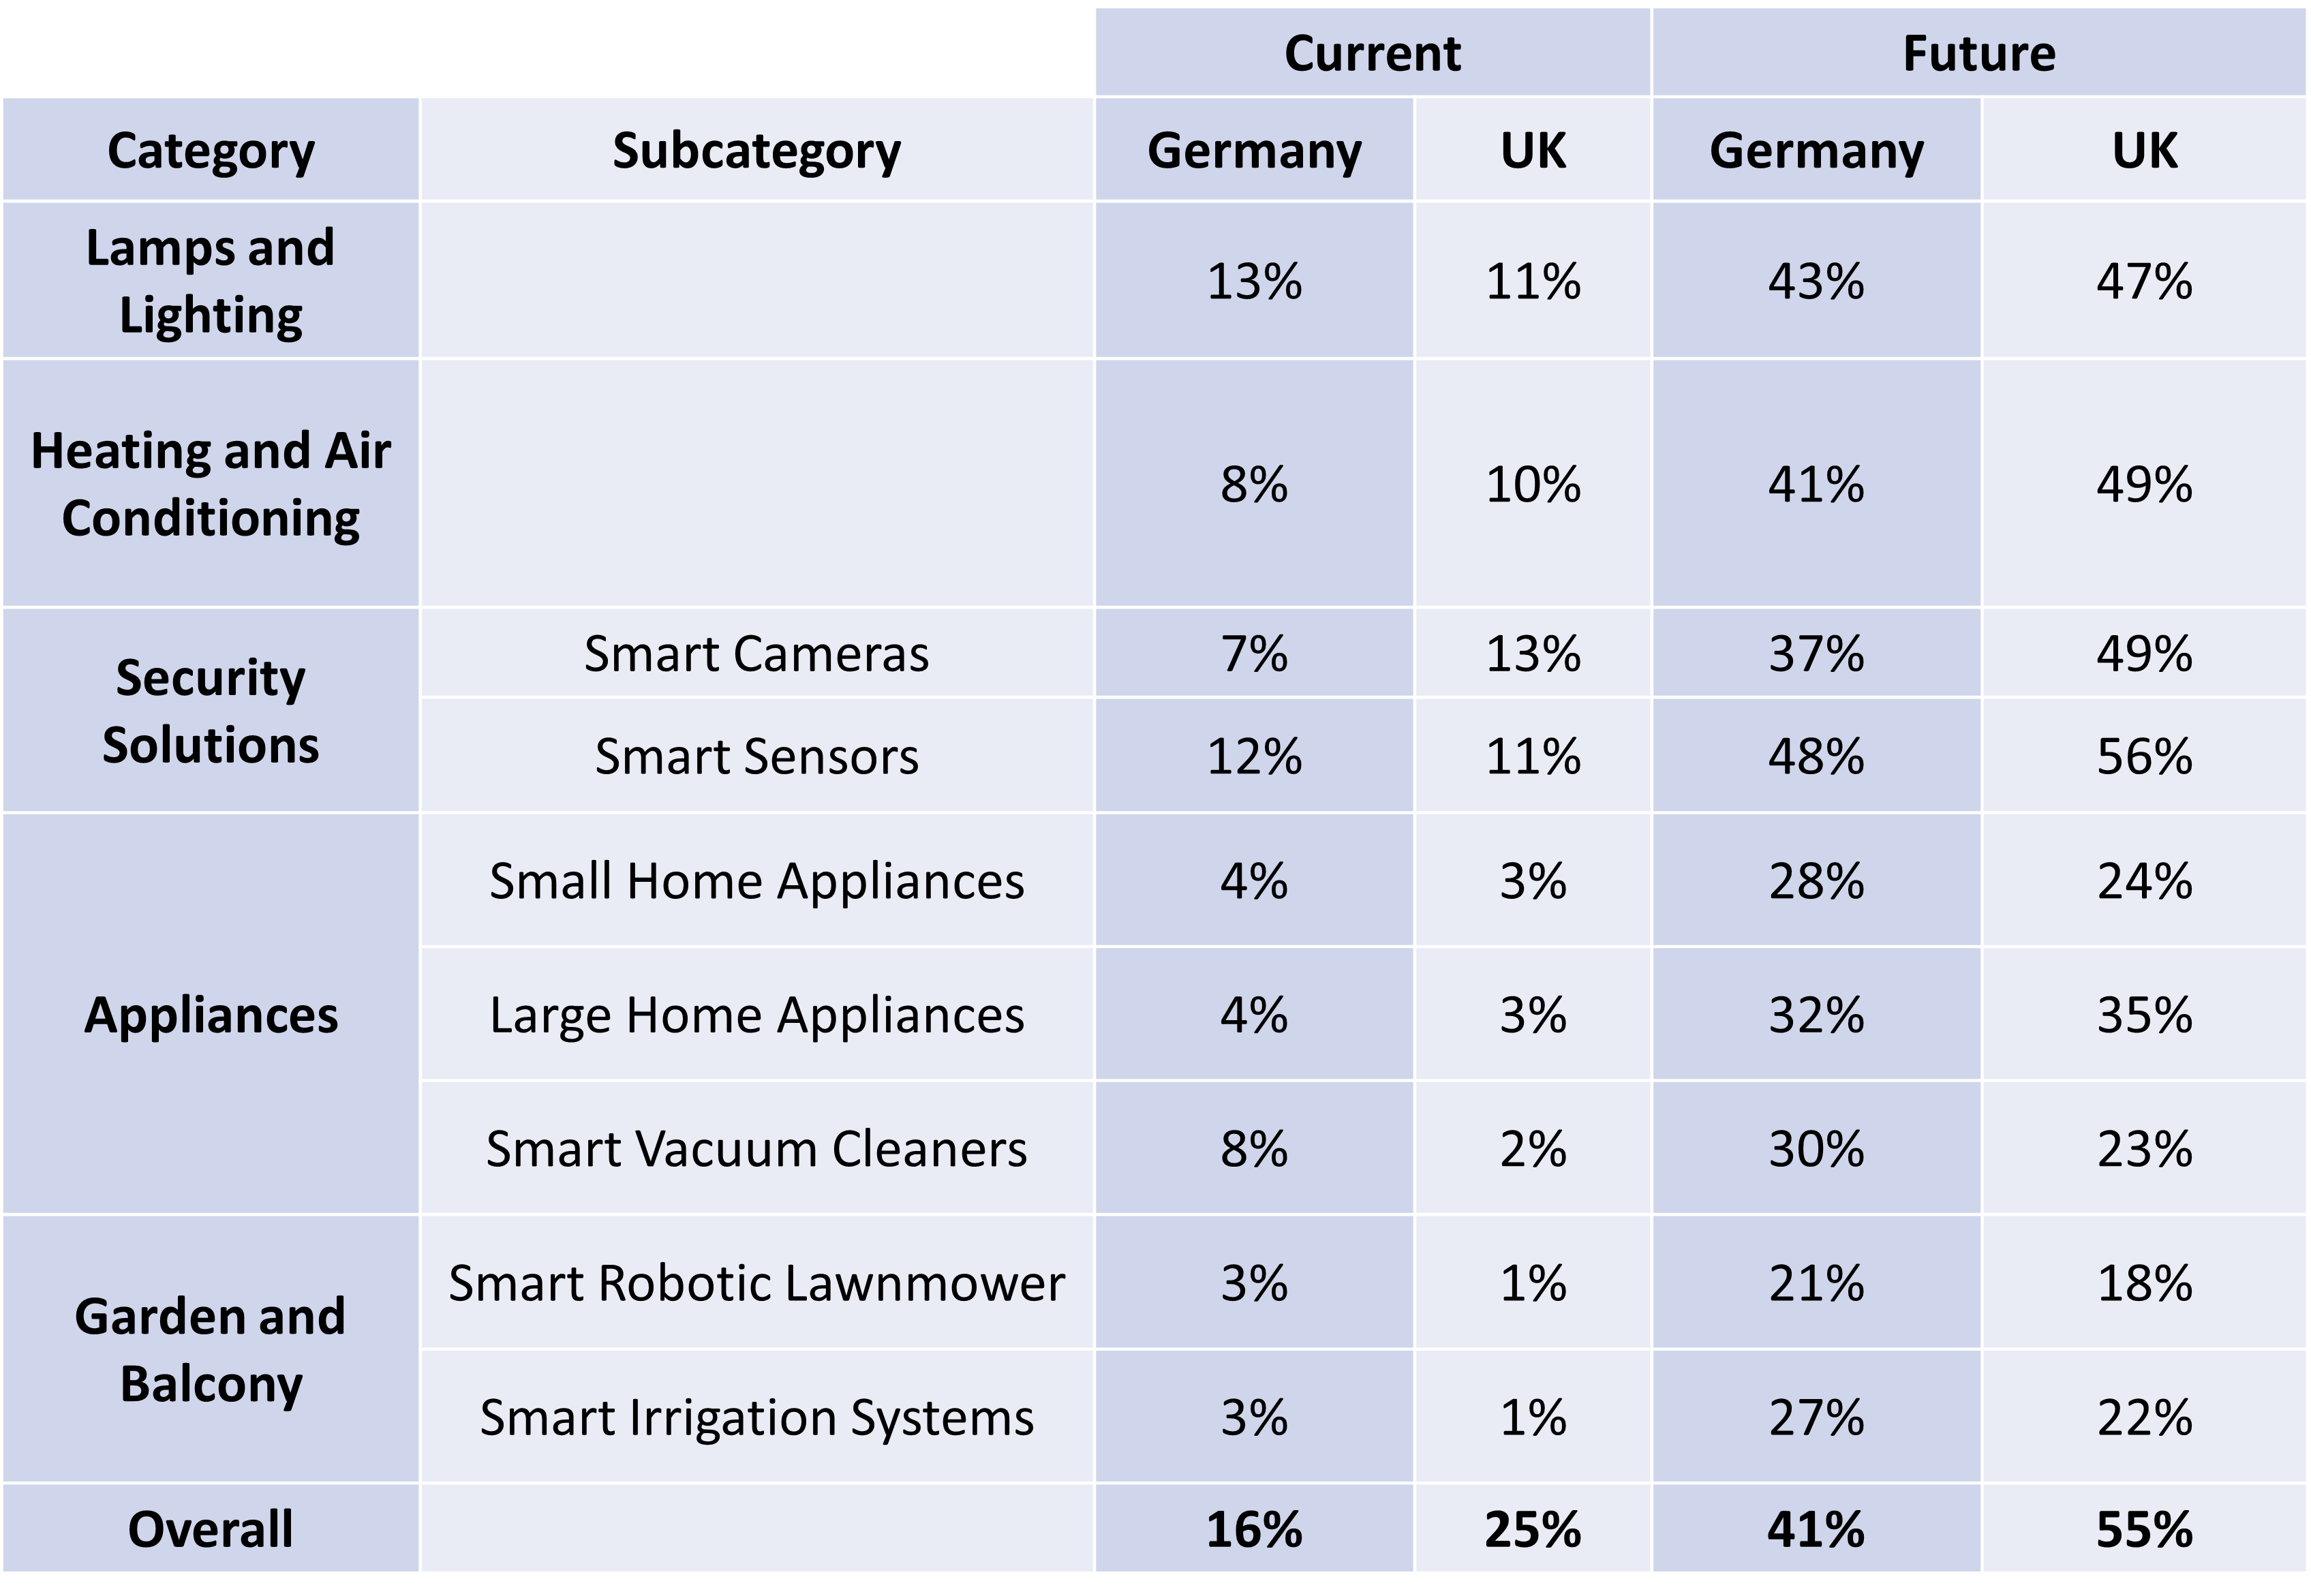
\includegraphics[scale=0.5]{assets/IoTTable.png}
\centering
\caption{Results of a Survey Regarding IoT Devices in Households Based on Data in Germany and the UK.}
    \label{table:IoT}
\end{table}



\subsection{Architecture}
\cite{article:Lombardi2021} published an article on a general overview between architectures, protocols and applications of IoT. The authors presented three different architectures that are most commonly found in the literature. 

The first architecture is a generic high-level architecture consisting of three layers, namely perception, network and application. The perception layer is the physical layer that interacts with the environment through information gathering and processing. Objects with computing power and the ability to interact with the outside world are an integral part of this layer. The network layer is the communication layer responsible for transferring data from the perception layer to the application layer. This layer includes all protocols and technologies required for this connection. An example of a protocol is 6LoWPAN, which stands for IPv6 over Low power Wireless Personal Area Network. The personal area network connects devices in a user's immediate environment, such as Bluetooth headphones with a mobile phone \cite{website:cloudFlarePAN}. The final layer is the application layer, which contains the essential software for a specific service. The data from the preceding layers is stored, processed, aggregated and filtered in this layer. The processed data is then made available to the IoT application.  

The second architecture is the service-oriented architecture. This architecture extends the three-tier architecture by adding a service layer between the application layer and the network layer. This service layer provides services to support the application layer and consists of several sub-services. The goal of this service-oriented architecture is to enable software and hardware reuse and to coordinate services. The architecture helps to connect different functional units through protocols and interfaces.   
% that are service discovery, service composition, service management, and service interfaces.


The third common architecture is the middleware architecture, also known as the five-layer architecture. This architecture is made up of five layers: the perception layer, the network layer, the middleware layer, the application layer and the business layer. The middleware layer, which aggregates and filters data received from the hardware, is an important layer. Various technologies are hidden in the middleware and standard interfaces are provided. This means that developers do not have to worry about compatibility between the infrastructures and the application and can therefore focus on the application development. 

The three architectures discussed can be seen in Figure \ref{graphic:IoTArchitecture}. Some additional architectures that also exist are the cloud-based architectures or the edge computing-based architectures.  



\begin{figure}[tph]
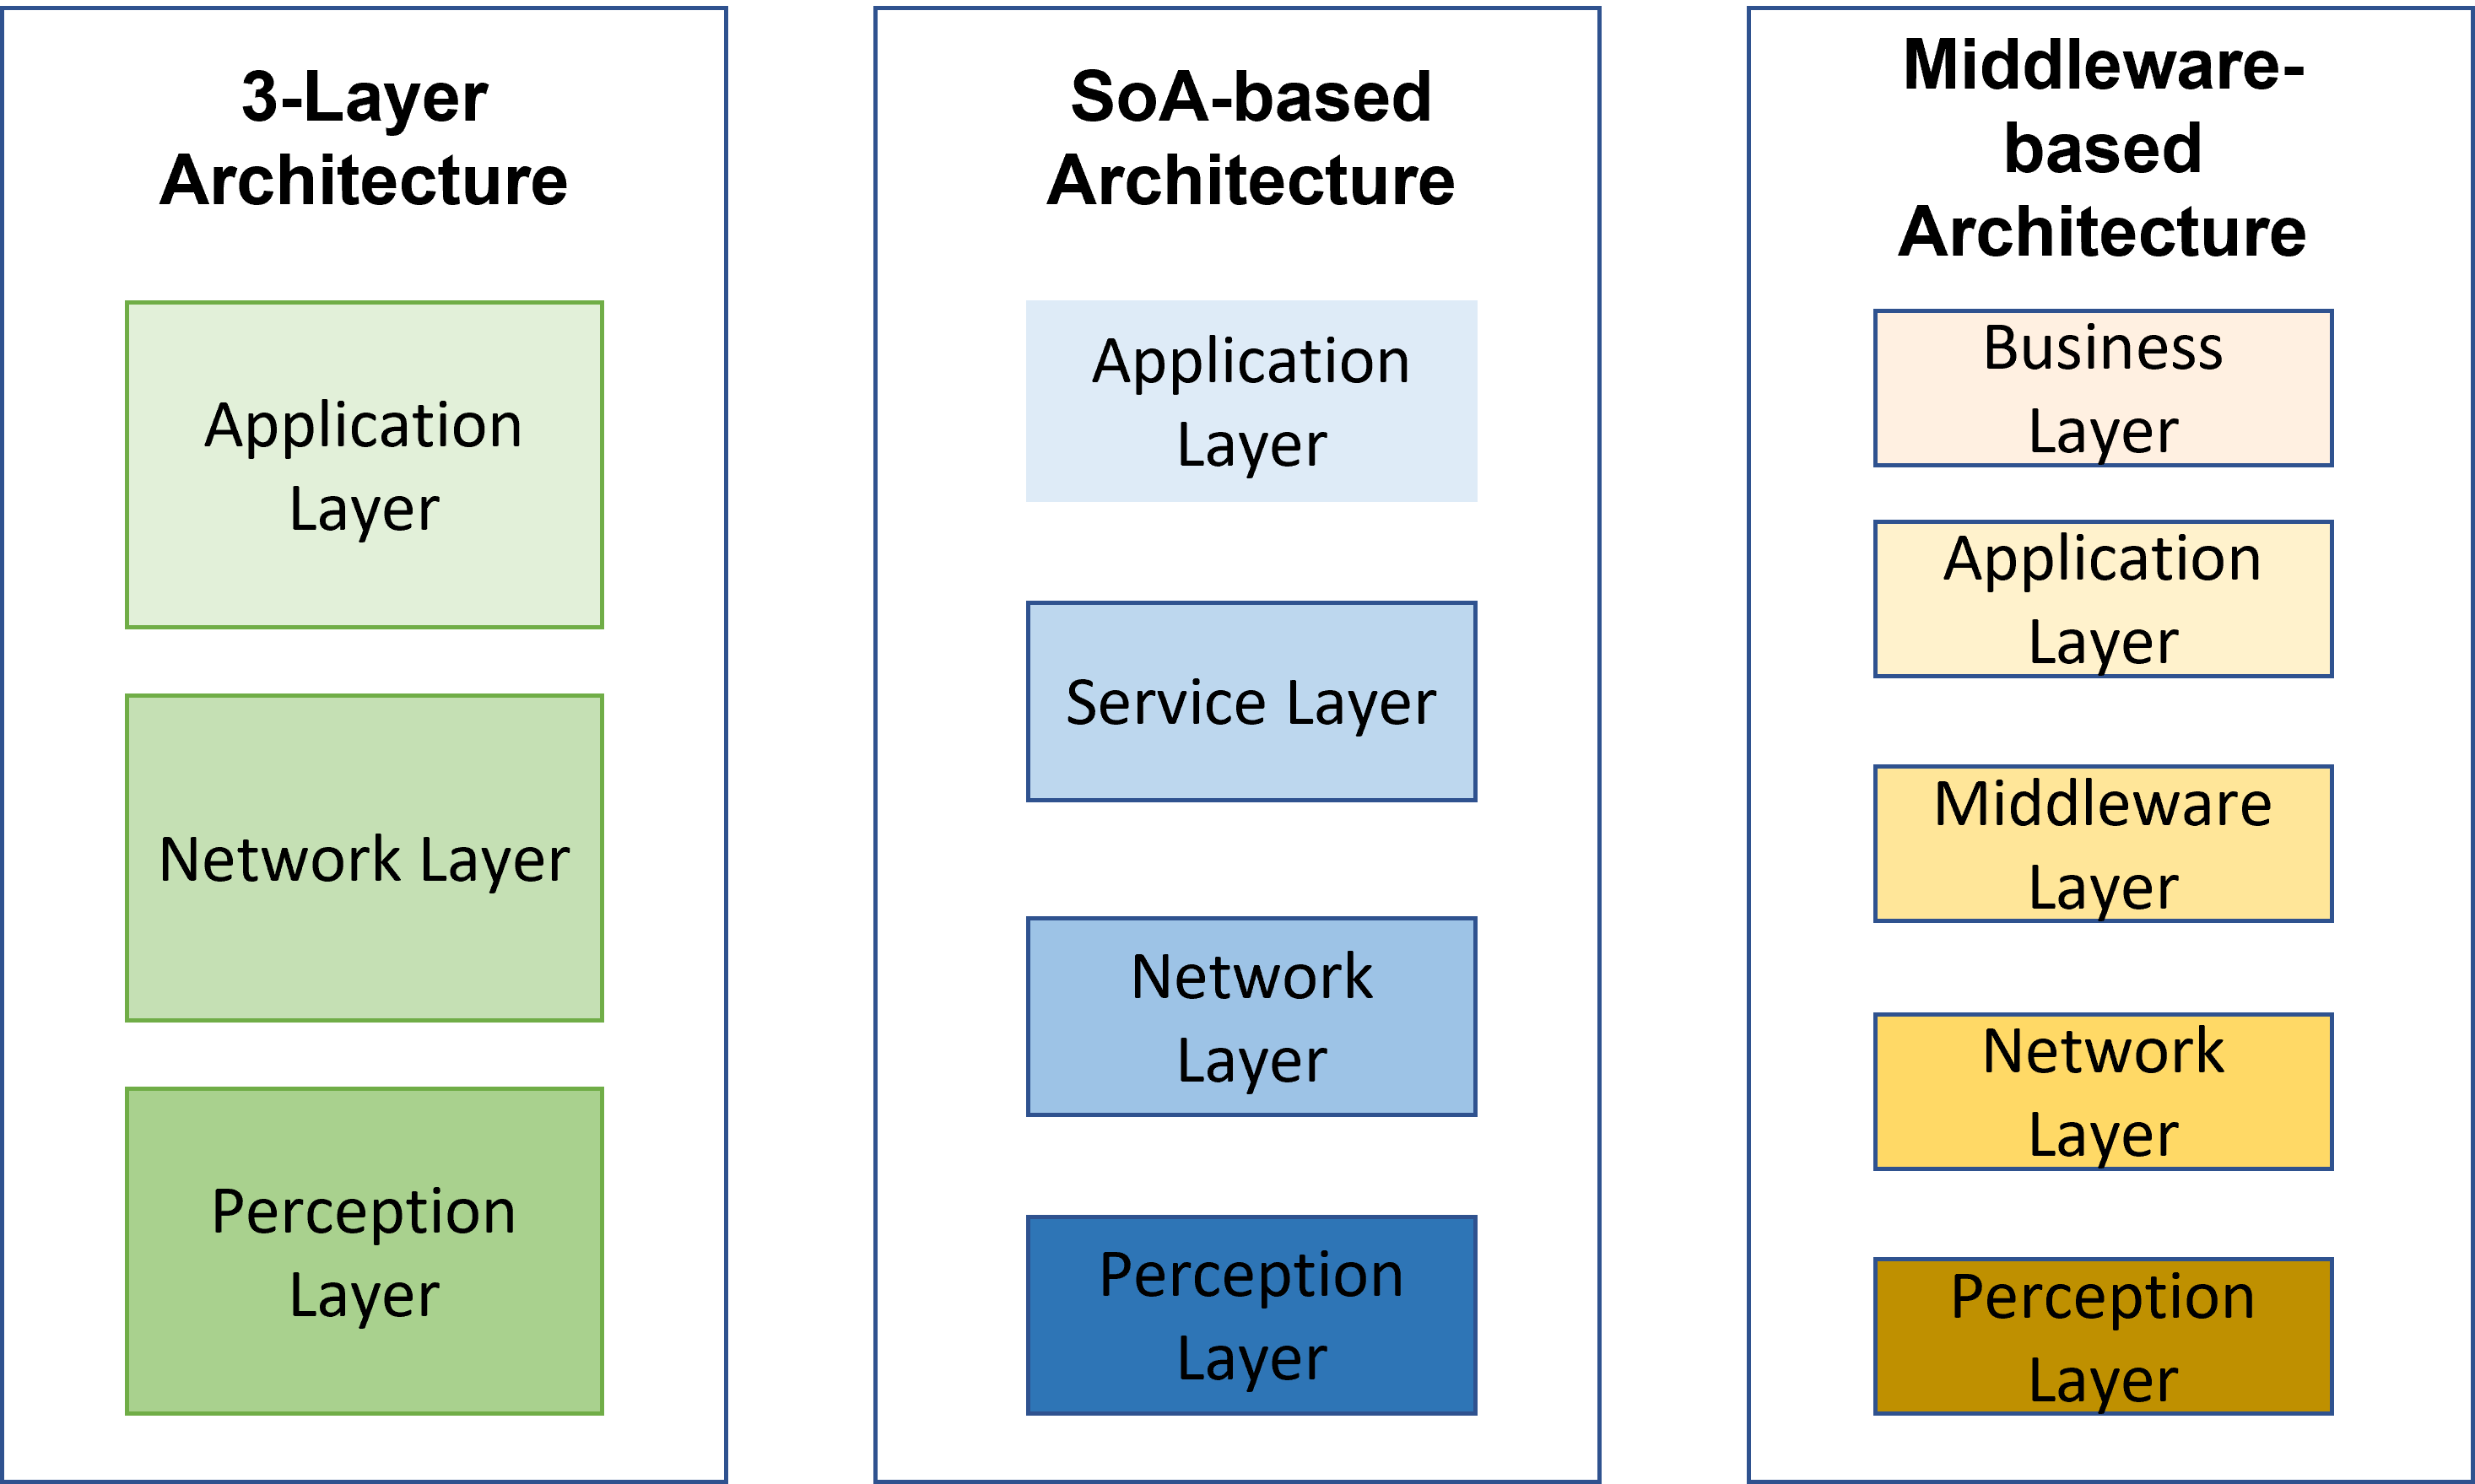
\includegraphics[scale=0.5]{assets/IoTArchitectures.png}
\centering
\caption{The Three Most Common IoT Architectures \cite{article:Lombardi2021}.}
\label{graphic:IoTArchitecture}
\end{figure}


\subsection{Hardware and Software Details of IoT} \label{sec:hardSoftware}
\cite{website:eclipseIoT} published a report on an IoT \& Edge Developer Survey with interesting insights. This survey was conducted in 2022 and 910 developers, committers, architects and decision makers were interviewed. One of the key findings for this thesis was that security concerns have almost doubled this year and are now in the top three challenges for developers, along with data collection \& analysis and connectivity. The most commonly used programming languages for constrained devices are Java, C and C++. In terms of the operating system (OS) for constrained devices, Linux distributions are the top choice with 43\%. FreeRTOS is in second place with 22\%. FreeRTOS is a real-time operating system for microcontrollers that is freely distributed under the MIT Open Source Licence~\cite{website:freeRTOS}. In third place is No OS/bare metal for constrained devices. The Linux operating system is further broken down into its distributions. Ubuntu makes up 23\% of all Linux operating systems, the second distribution is Raspbian with 20\%, the third is Alpine with 18\% and the fourth is Debian with 17\%. Interestingly, there are many more distributions in use, but they have a maximum share of 13\%. This information can be seen graphically in \ref{graphic:IoTOSs}.


In terms of architecture for constrained devices, ARM dominates. The most common architecture is ARM Cortex-M0/m0+ with 26\%. ARM Cortex-M3/ARM Cortex-M4 follows with 24\%. In third place is the ARM Cortex-M7 with 20\%.  




\begin{figure}[tph]
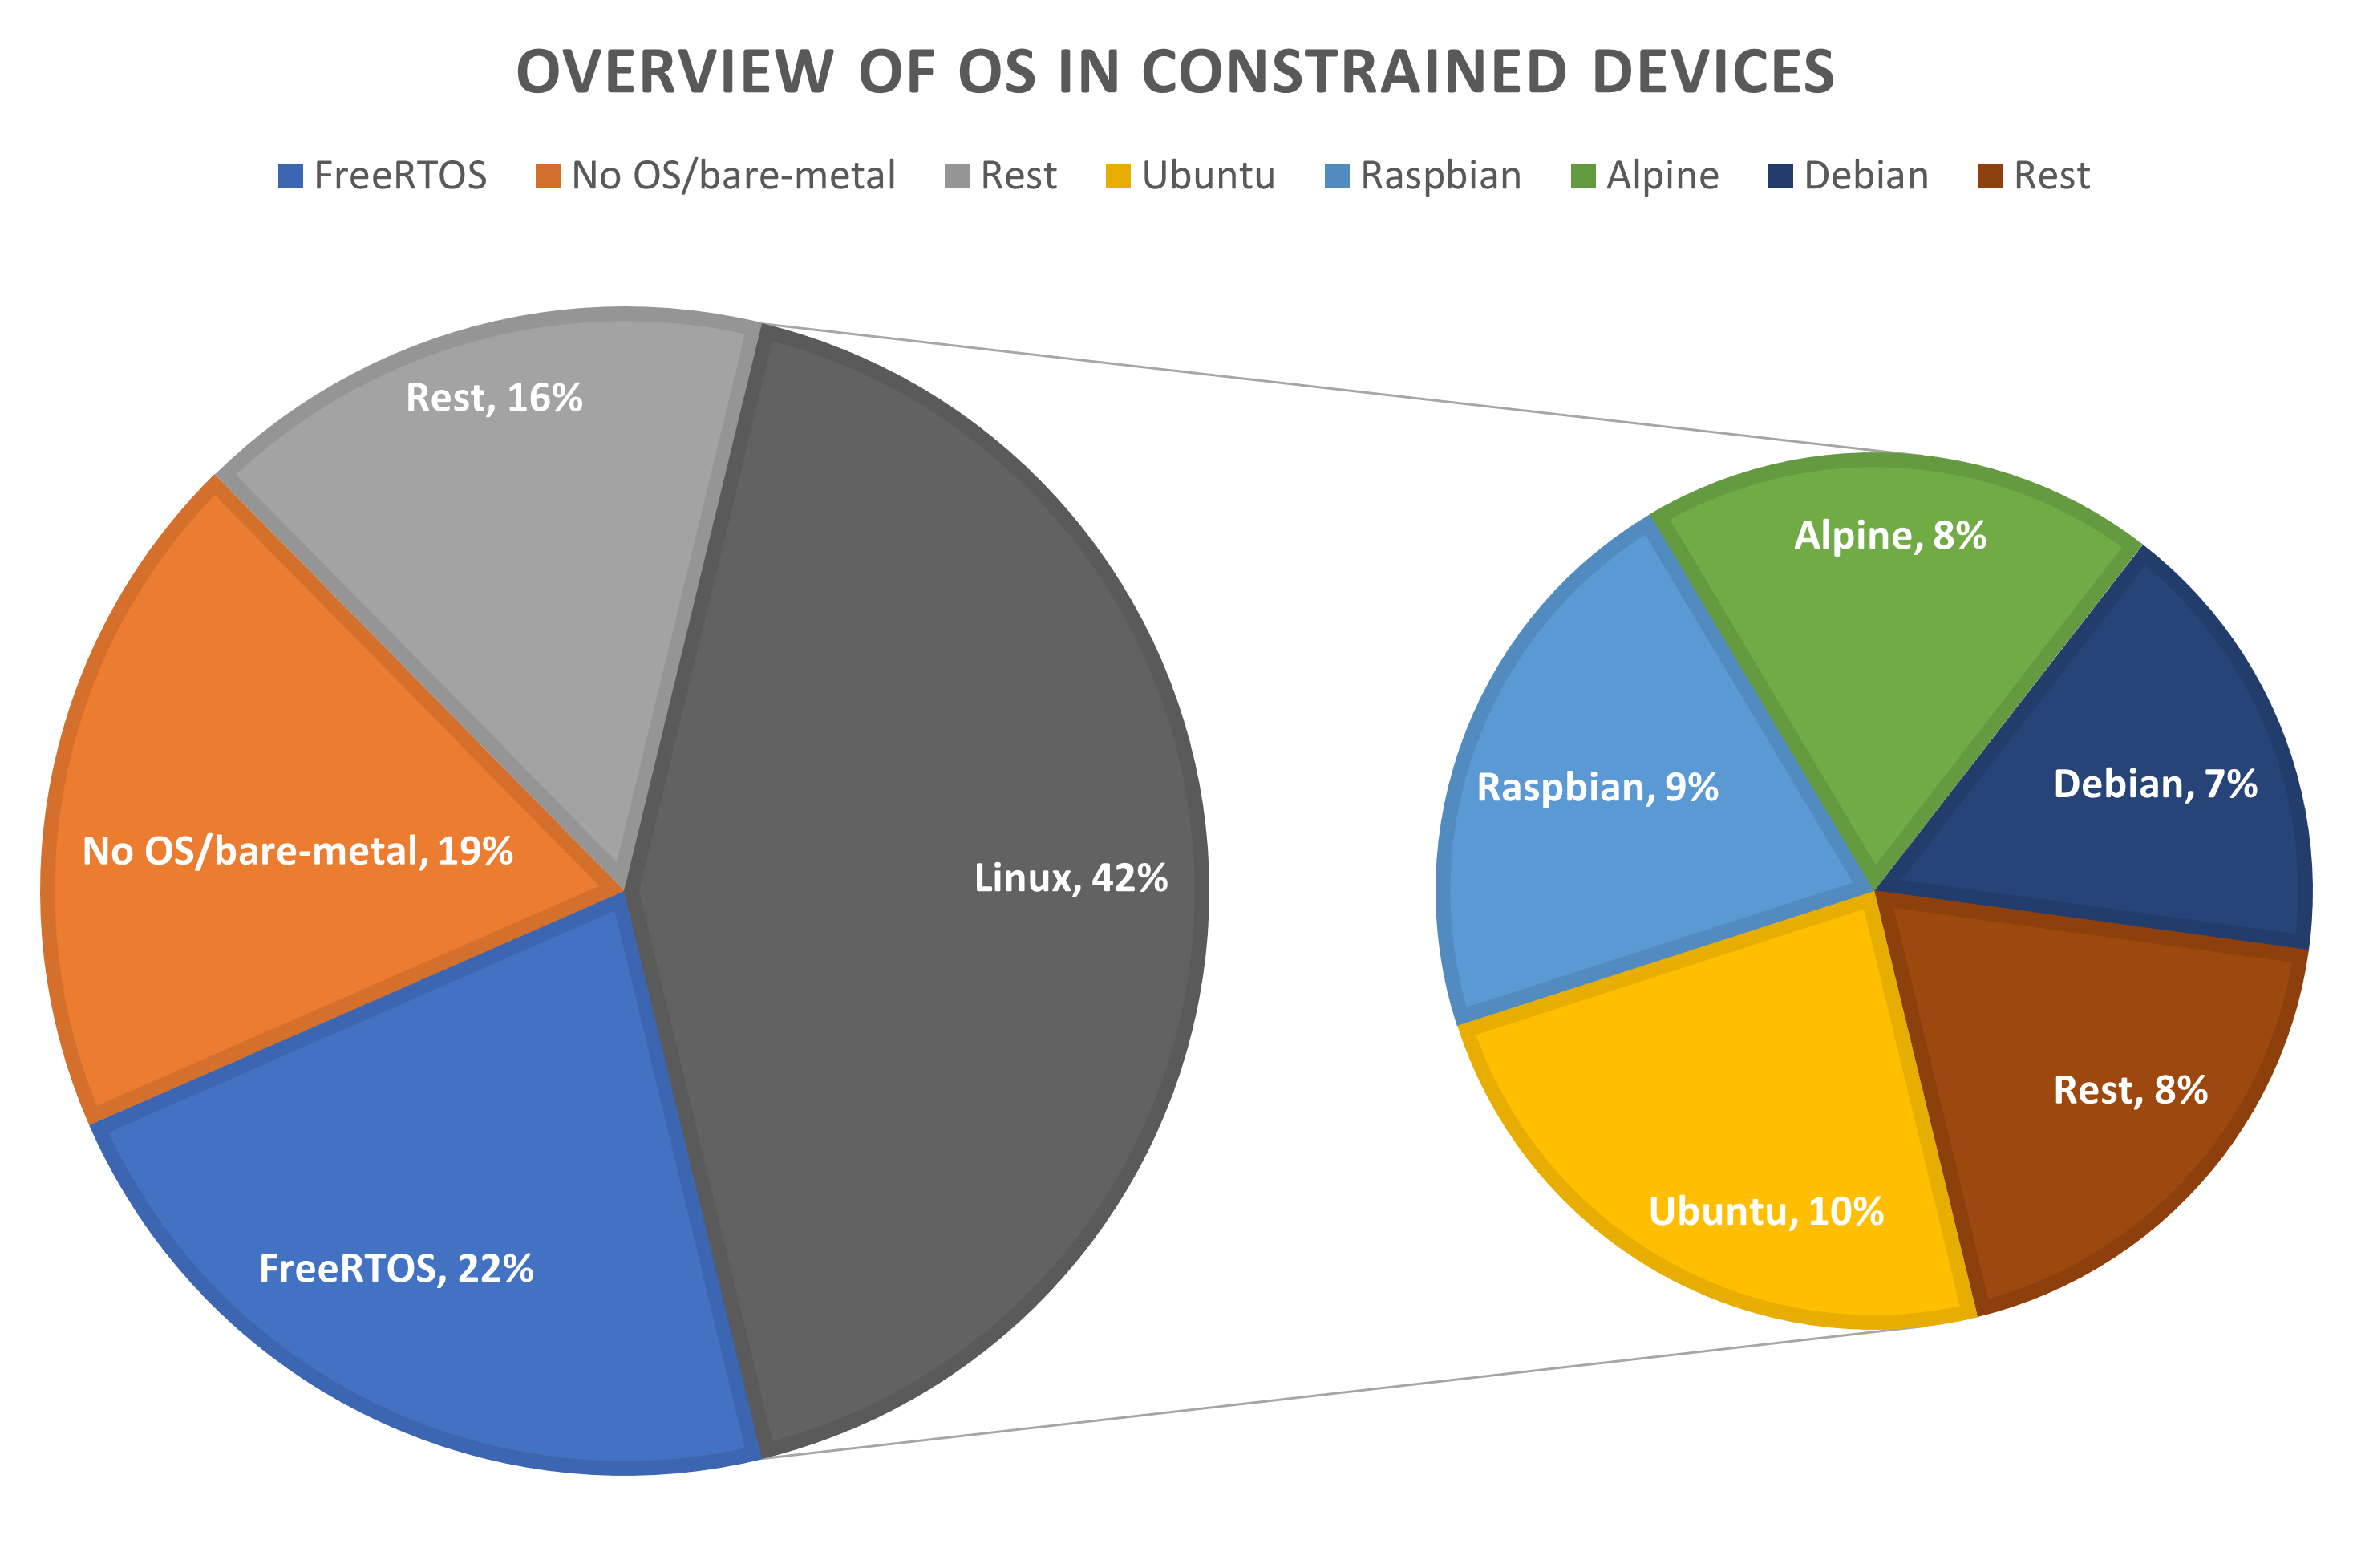
\includegraphics[scale=0.55]{assets/IoTOS.png}
\centering
\caption{The Most Commonly Used OSs in Constrained Devices.}
    \label{graphic:IoTOSs}
\end{figure}





\section{Malware and IoT} \label{section:MalwareAndIoT}
This section gives a general overview of malware, especially in the context of IoT devices. A more detailed analysis can be found in Section \ref{main:bashlite}, where Bashlite is analysed.

Malware or malicious software is a term used to describe malicious code or a program that is harmful to a system~\cite{website:malwarebytes}. Examples of malware or malware families related to IoT are Mirai, Bashlite, Tsunami or Hajime~\cite{article:surveyIoTmalware}. Mirai and Bashlite are probably two of the best known examples. Mirai, for example, was still highly prevalent in the first quarter of 2019~\cite{website:KasperskyAMalwareStory}. Bashlite, also known as Gafgyt~\cite{website:TrendMicroBashlite}, was already much less common in 2019~\cite{website:KasperskyAMalwareStory}, but other malware such as Mirai has inherited 
 from its source code~\cite{article:surveyIoTmalware}.

 
\cite{article:evOfBashlite} gave a brief overview of Bashlite and Mirai and how they are used to create botnets. The rest of this paragraph is based on that article.
Since the source code of Mirai is based on that of Bashlite, they share some similarities. For example, both infect IoT devices that can be accessed with known and/or vulnerable authentication credentials. They also both aim to create botnets. These botnets have different components. The command and control (C\&C) servers send commands to the infected devices and essentially act as the operator's interface to the botnet. The bots are the infected devices that make up the botnet. They execute the commands received from the C\&C servers. There are also scanners that identify vulnerable devices by looking for Telnet and SSH servers that the scanners attempt to log into. Loaders download and run the malware of the botnet after logging into the vulnerable devices. Malware servers provide resources such as executable binaries to the botnet. A possibly distributed database stores collected information such as scan results or active bots.

Such botnets can be used for different purposes~\cite{website:IBMIoT}, which  are described below. The first purpose is the aforementioned DDoS attack. The idea is to attack a target by sending so much traffic from many different machines that the target cannot handle the volume, eventually taking the target down. Another use for botnets are spam bots. Using botnets, spam can be sent from IP addresses that are not yet known to be spam relays and therefore not yet blocked by system administrators. A third purpose are crypto mining bots, which can be used to mine cryptocurrencies such as Monero. These malware require a device with sufficient processing power (e.g. smartphones), so constrained devices are not optimal for such malware to infect.

According to~\cite{article:DDoSinIoT}, there are five main reasons why IoT devices are advantageous for creating botnets:
\begin{itemize}
\item IoT devices often operate around-the-clock, they do not have on-off cycles like laptop and desktop computers. 
    \item IoT devices are poorly maintained. A very common problem is that devices are set up and then forgotten about as long as they are working properly. 
    \item IoT devices are capable of generating significant distributed denial of service (DDoS) attack traffic, similar to the attack traffic generated by modern desktop systems. 
    \item IoT devices are often either non-interactive or require minimal user intervention, resulting in infections going unnoticed. 
\item IoT vendors favour usability and user-friendliness over security, resulting in weak protection.
\end{itemize}

The last item in the enumeration includes a number of known vulnerabilities~\cite{website:IBMIoT}. The first are weak passwords to make it easier to set up and use the device. These passwords are many times printed in the user manual or even outside the packaging. As the credentials are often the same for all the same devices, this is a huge problem. Even if the credentials were not so accessible, they are often predictable combinations such as "admin/admin". In addition, many devices lack encryption. Such security features are often not even considered. In addition, vendors sometimes add hidden access mechanisms, called backdoors, to devices. They might do this to make it easier to support the device, but it could also be used by hackers. An example is an open port on the device that cannot be closed. 


\subsection{IoT Malware Statistics}
\cite{website:KasperskyAMalwareStory} published a report in which the authors researched attacks on IoT devices using honeypots. The authors mentioned that such honeypots are the best option to track attacks, catch malware or just get a general overview. This subsection is based on that source. There exist three different common types of honeypots. 

\begin{itemize}
    \item Low-interaction honeypots simulate services such as SSH, Telnet and web servers. The attacker is fooled into thinking that this is a real susceptible system and attacks the honeypot.
    \item High-interaction honeypots are real systems that have the advantage of running fully POSIX capable systems. POSIX is a standard defined by the IEEE~\cite{website:IEEEPosix}. This standard helps to maintain compatibility between operating systems~\cite{website:linuxHint}. As these honeypots are real systems, it is important to take action against the malicious activity of the malware (e.g. prevent further systems from being compromised). 
    \item Medium-interaction honeypots are a combination of low-interaction and high-interaction honeypots.  
\end{itemize}

The authors collected data from more than 50 honeypots around the world over the course of more than a year.

In the first six months of 2019, the Telnet honeypot detected more than 105 million attacks from 276,000 attacking IP addresses. This is significantly more than the 12 million attacks from 69,000 IP addresses in the first half of the previous year. The most attacking IP addresses came from Brazil and China with 30\% and 19\% respectively. Egypt, Russia and the US followed with 12\%, 11\% and 8\% respectively. Regarding the top malware threats that attacked the Telnet honeypot, 6 out of 10 were Mirai variants. There are several reasons for this, including the public availability of the malware and its ability to create bots of any complexity and for any hardware configuration. The NyaDrop family of malware was the most common, accounting for around 39\% of all attacks. This is a Linux trojan that targets IoT devices and specifically the MIPS CPU architectures~\cite{website:comodoAntivirus}. In second, third, fourth and fifth place were the Mirai variants with 22\%, 12\%, 2\% and 2\% respectively. 

Another interesting finding was the most common combination of credentials tried. "support/support" was tried 2,627,805 times, "root/vizxv" was tried 2,376,654 times, and "admin/admin" was tried 2,359,985 times in the first quarter of 2019. The second is the default combination for connecting to a vulnerable camera from Dahua via Telnet~\cite{website:dahuaDefault}. The last interesting finding the authors made was in terms of the ports targeted by the malware. TCP ports were clearly the most targeted, with only a small number of attacks targeting ICMP and UDP ports. Unfortunately, the authors did not provide statistics for other protocols such as SSH in the same depth as they did for the Telnet protocol.  


\subsection{P2P IoT Botnets} \label{subsection:P2PIoTBotnets}
The botnets described so far correspond to the typical IoT botnet~\cite{website:trendmicroTheFuture}. Adversaries control the botnet from a C\&C server that controls various infected devices. This means that taking out the C\&C servers renders the entire botnet useless, regardless of how many bots are connected to the system~\cite{website:trendmicroTheFuture}. While taking down many C\&C servers can be cumbersome, it can also be a convenient solution against botnets. For example, this strategy was used against the Andromeda botnet~\cite{website:europol}. Several international authorities took action against domains and servers that were spreading the Andromeda malware. This involved, for example, sinkholing  1500 domains. Sinkholing is when traffic is redirected to a server other than the intended one, such as one controlled by law enforcement authorities~\cite{website:europol}. 
However, this solution vanishes as soon as the botnet is set up as a peer-to-peer (P2P) network.~\cite{website:trendMicroUncleanable} wrote a technical briefing on the development of IoT botnets in combination with P2P networking. The rest of this subsection is based on that source.

Unlike a botnet with a central server, a P2P network is much more robust. The authors use BitTorrent as an example because it has withstood the test of time, having been used to share illegal content for over 20 years without the authorities being able to shut it down. In the case of a P2P IoT botnet, each bot would need to be disinfected separately, as there is no central server. This is also a problem caused by the insecurities of IoT systems, as discussed in Section \ref{section:MalwareAndIoT}. In the case of a desktop environment, mass cleanup would theoretically still be possible, e.g. by antivirus vendors, but this is not an option for IoT devices because there is no antivirus protection. Fortunately, there are not many P2P botnet families yet, the authors stated that they have only seen five families so far, and they also suspect that they are not common at the moment. Although they do not know the actual number of infections, they find it worrying that the rate at which P2P botnet malware appears is increasing. The authors conclude that this indicates an increased interest in creating P2P botnet malware. The authors then briefly describe each of the five malware families. One of these five is described below to give a general idea.

The most recent malware mentioned by the authors is "HEH". HEH is written in Go and scans and infects via Telnet port 23 and port 2323 with hardcoded credentials and brute-forced passwords. The malware starts by randomly selecting an IP address and then uses an algorithm to derive the P2P port from that IP address. Thus, no list of IP addresses and ports is required. Once a victim is infected, it attempts to connect to other peers. Additionally, the malware stops the HTTP service and starts its own service instead, which acts as a download site for infected devices. The P2P protocol has 5 operation codes, 4 of which are for synchronisation and one for receiving commands. The latter accepts various instructions such as 'exit', 'attack', 'execute' and 'self-destruct'. According to the authors, the last command was particularly interesting because it is unusual for a bot to be able to destroy itself.


The authors also shared their thoughts on the future development of P2P IoT botnets. They emphasized the importance of making money as an incentive for cybercriminals to develop malware. Since these incentives are critical to development, it makes sense to take a look at how these incentives have evolved.
Routers are an interesting target for attackers because they act as an entry point into a home network. An infected router also offers many opportunities such as man-in-the-middle attacks or information theft. Additionally, an infected router allows lateral movement to infect other unsecured devices on the network. The authors also mentioned that, in terms of financial incentives, a distinction needs to be made between the pre-Covid 19 era and now, due to the increase in home offices. For example, an infected home router could now be an entry point into a company, which could be a possible financial incentive for adversaries. There is also a general risk that a successful attack will motivate other cybercriminals to do the same. For example, the authors predict that once a P2P IoT botnet is successful enough, all other botnets will start using P2P capabilities as well.
As a result, there is a realistic risk that such P2P malware will be further developed and distributed, but this is highly dependent on the financial incentives.

As this chapter has shown, there are many problems with the security of IoT devices. There are several reasons why IoT devices are susceptible to malware, such as poor maintenance or a focus on usability rather than security~\cite{article:DDoSinIoT}. Infected IoT devices can be used for malicious behaviour. One problem are botnets, where infected devices act as bots that execute commands sent by an adversary. As~\cite{website:KasperskyAMalwareStory} noted, there were about 9.5 times more attacks in the first half of 2019 (105 million) than in the first half of 2018 (12 million), which is an extreme increase. Another growing problem are P2P IoT botnets. Even if they are not very prevalent currently, it is certain that these P2P botnets can become a major threat in the future because they are almost unkillable. Each of the above points makes it clear that a way to defend against such threats is essential.



\section{Cooperative Defense}
There were not many resources available on the subject of cooperative defence. The ones found are presented in this section.

\cite{article:Zhang} is a relatively old paper from 2005 in which the authors aim to detect DDoS attacks in the intermediate network. The goal was to enable a DDoS attack detection system to share information, rather than to improve a currently available detection method. To achieve this, they proposed a dynamic defence infrastructure consisting of independent defence nodes and assumed that a DDoS attack heading towards a victim would consume more bandwidth than a normal use of the Internet. For scalable and resilient communication to exchange attack information, the authors designed a directional gossip mechanism. Each defense node sets a limit on the amount of traffic it deems malicious, based on its own defense strategy. This usually results in a high number of false positives due to the dynamic nature of the Internet. The defense accuracy is improved by the gossip mechanism, which helps to transmit information between nodes. During this information exchange, the rate limit is adjusted at each individual defence node.
When the mechanism for aggregating information converges, the defense node's rate limit will have roughly global information of the attack, which allows it to more accurately block/drop malicious traffic.


\cite{article:RodiguesBlockchain} and~\cite{article:RodriguesEvaluation} proposed and evaluated a cooperative defence mechanism based on the blockchain. The authors presented a scenario in which a web server in an autonomous system is under a DDoS attack from devices hosted in other autonomous systems. An autonomous system is a network or group of networks which share a single routing policy~\cite{website:cloudFlare}. A routing policy contains a list of IP addresses controlled by the autonomous system and a list of other autonomous systems to which it is connected~\cite{website:cloudFlare}.
In this scenario, the web server relies on the defences of the autonomous system where the server is located. As it is better to block malicious traffic close to its origin, this approach is not ideal. This is where the blockchain comes in. The idea is to store the attacker's IP address in a smart contract created by the collaborative defence participants. In this way, subscribed autonomous systems on the Ethereum blockchain receive an updated list of addresses to be blocked and also confirm the authenticity of the attack. Once the other autonomous systems receive the updated list and confirm the attack, the mitigation strategies in the autonomous system can be triggered to block malicious traffic close to its origin.


